\documentclass{HZNUMCM}
\setControlNumber{888888}
\setContestType{ICM}
\setProblemLetter{A}
\setPaperTitle{my title}
\setBibFilename{paper.bib}
\setSummary{hkshjjlghjgkl;dfcgvhjkl;\\
	\controlnumber ~for \contesttype\\
	\\ dfghjkl sdffasfas fas fas fas fas f as fas f sadf as fa sdf as f asf a f as fa sf as fa sf s fs f as fas   \begin{equation}
		\int_a ^bf(x)dx=0
	\end{equation}
f as fa sf a fds f 

	\indent\indent fdskkfsdfjlsd }
\begin{document}
\showSummarySheet
\showContents

\section{Introduction}
\subsection{Problem Background}
Taking a bath is a daily activity to remove the stains and have a rest, the cooling of water during 
a bath has always been a big problem for our bathing experience. Of course it is perfectly possible
to live a full and active life without knowing anything about bathing strategy at all. But how could
we improve the quality of life through taking a better bath?

To solve this problem,  we need to construct the time-space based bathtub temperature model to
determine the optimal strategy which could achieve the following three objectives:
\begin{enumerate}[\quad\bf1.]
    \item To keep the temperature \textbf{even} throughout the bathtub;
    \item To keep the temperature as close as possible to the \textbf{initial} temperature;
    \item \textbf{Not to waste} the water too much.
\end{enumerate}

\subsection{Our work}
\begin{enumerate}[\bf 1.]
    \item We construct a time-space based temperature model to research the change of the
    temperature in the bathtub.
    \item We use free cooling process to test some unknown parameters' value.
    \item Through controlling the change of the inflow temperature and flux, we make some effective
    strategies to meet the demand of optimum and uniform temperature in the bathtub.
    \item In order to examine the extent of our model, we test whether good strategies in the
    initial model still have the same effect on the model which changes some parameters based on
    normal bathing.
\end{enumerate}

\section{Preparation of the Models}
\subsection{Assumptions}
It is difficult to study the actual situation in the bathtub because of the complex principles about
water-flowing and the heat conduction. In order to simplify the problem and to hold the correctness
of results at the same time, we make the assumptions below to simplify the bath
problem:
\begin{enumerate}[\bfseries 1.]
    \item We ignore the loss of water through evaporation. According to \cite{2011_Ozturk_1532,2010_nakata_MR2680013,2009_li_R2451705,2009_muroya_MR2481600}, the evaporation
    capacity of water is only about $7.35\times10^{-8}$m/s, so it is a tiny quantity of the whole
    water.
    \item We ignore the influence caused by different density of cold and hot water(such as the
    flow) in order to simplify the model, and with the consideration that people may move around in
    the bathtub.
    \item Our model concentrates the bathtub with full water, which can eliminate the effect of the
    overflow drain.It is based on the consideration that the change of position is difficult for
    liquid, and the change of temperature in water is smooth (That is to say the excess water is
    almost the same with the upper water).
\end{enumerate}

\subsection{Notations}
The primary notations used in this paper are listed in \textbf{Table \ref{Ntt}}. There can be some
other notations to be described in other parts of the paper.
\begin{table}[!htbp]
\begin{center}
\caption{Notations}
\begin{tabular}{cl}
    \toprule
    \multicolumn{1}{m{3cm}}{\centering Symbol}
    &\multicolumn{1}{m{8cm}}{\centering Definition}\\
    \midrule
    $I$&The Intensity of the Heat Source\\
    $k$&The Material's Conductivity\\
    $h$&The Heat Transfer Coefficient\\
    $c$&The Heat Capacity of Water (=4200 J/(kg$\cdot^\circ$C))\\
    $\rho$&The Density of Water (=10$^3$ kg/m$^3$)\\
    \bottomrule
\end{tabular}\label{Ntt}
\end{center}
\end{table}

\section{Time-space Based Temperature Model through PDE}
\textbf{Partial Differential Equation Method} (\textbf{PDE-Method}) \cite{2011_Ozturk_1532} is very useful in
solving the problems about the variables changed both by position and by time. In the problem of the
heat conduction in bathtubs, it is proper to use such a kind of method to find out the temperature
distribution in a bathtub in different time points.

We use \textbf{PDE-Toolbox} in \textbf{MATLAB} software to solve the model of temperature
distribution in the bathtub. \textbf{Figure \ref{jj}} shows the structure of our model, which can be
divided into two parts: \textbf{PDE Solving Model} and \textbf{Analysing Model}. The former helps us
to get the temperature distribution in the bathtub in different situations, and the latter helps to
decide which strategy is better for an joyful experience while bathing.
\begin{figure}[!htbp]
    \small
    \centering
    \includegraphics[width=14cm]{model.jpg}
    \caption{The Structure of Model}\label{jj}
\end{figure}

\subsection{Construction of PDE-Solving Model}
In order to construct a model more close to the normal condition, we need to establish a
\emph{particular} bathtub with some actual parameters and make some preparations for the initial and
optimum temperature. For an established condition of bathtub with specific faucet and inflow, we can
use some laws about heat transmission to analyse the state of the water, such as the temperature and
its stability.

\subsubsection{General Preparations for PDE Solving Model}
We decide a typical bathtub for our research. \textbf{Table \ref{tb1}} shows the size of the
bathtub, together with the size of the human body settle in the bathtub (also very typical) and the
temperature in different situations.
\begin{table}[!htbp]
\begin{center}
\caption{The value of geometry size and temperature}
\begin{tabular}{lll}
    \toprule
    Class&Quantity&Value\\
    \midrule
    Size of the bathtub&Length&1.8m\\
    &Width&0.8m\\
    &Depth&0.6m\\
    \midrule
    Size of the human body&Length&0.8m\\
    (consist of two cubiods)&Width&0.2m\\
    \midrule
    Temperature&Human skin&36$^\circ$C\\
    &External (the wall and the air)&20$^\circ$C\\
    &The Water in bathtub&35$^\circ$C (Initial)\\
    \bottomrule
\end{tabular}\label{tb1}
\end{center}
\end{table}

The 3-D Model of the bathtub is shown in \textbf{Figure \ref{md}}.
\begin{figure}[!htbp]
\small
\centering
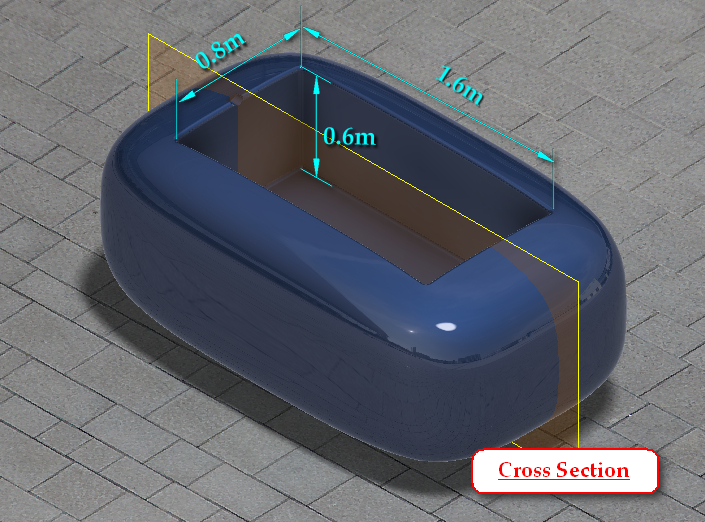
\includegraphics[width=12cm]{bathtub.png}
\caption{The 3-D model of the bathtub, designed with \emph{Inventor 2017}}\label{md}
\end{figure}

It is always difficult to study the 3-D space with PDE-Method. So in our study, we just research a
particular \textbf{cross section} of the bathtub which can represent the distribution of temperature
in the whole bathtub. The position of the cross section has been emphasized in \textbf{Figure
\ref{jj}}, and the component of the section is shown in \textbf{Figure \ref{cs}}.
\begin{figure}[!htbp]
    \small
    \centering
    \includegraphics[width=12cm]{sp2.png}
    \caption{The component of the cross section}\label{cs}
\end{figure}

\subsubsection{Partial Differential Equation of Heat Conduction}\label{k}
In order to calculate the change of temperature by time for each small water component, the
\textbf{Heat Conduction Equation} is needed. It can be expressed as
\begin{equation}\label{hc}
u_{t}=\frac{k}{\rho c}\nabla^2u+I,
\end{equation}
where
\begin{itemize}
    \item {$u_{t}$} is the temperature's derivative by time, which represent the change we want to
    know;
    \item $k$ is the thermal conductivity of water (W/(m$\cdot$K));
    \item $\nabla^2u=\mathrm{div}(\nabla u)$ roughly means the change of temperature in different
    positions;
    \item $\rho,c$  are the density and heat capacity of water, whose value has been given in
    \textbf{Table \ref{Ntt}}.
\end{itemize}

To set the value of $k$, we consider the theoretical basis of the Equation (\ref{hc}), \textbf{the
Fourier's Law}. The law states that the time rate of heat transfer through a material is
proportional to the negative gradient in the temperature and to the area, at right angles to that
gradient, through which the heat flows. It is shown as:
\begin{equation}
\vec q=-k\nabla T
\end{equation}
where (including the SI units)
\begin{itemize}
    \item $ \vec q $  is the local heat flux density (W/m$^2$);
    \item $k$ is the material's conductivity (W/(m$\cdot$K));
    \item ${\nabla T}$ is the temperature gradient (K/m).
\end{itemize}

The thermal conductivity $k$ is often treated as a constant, though this is not always true. When
water is absolutely static, the value of $k$ is very little. However if the value of $k$ in static
condition is used in the model, a bathtub of water can keep the temperature for even 10 minutes! The
reason for this is that the water flow can carry much energy. Therefore we set:
\begin{equation}\label{u}
k=0.6+M(\max u-\min u).
\end{equation}
The first term is water's initial thermal conductivity \cite{2011_Ozturk_1532}. The second term is to reinforce
the influence of water flow, where the coefficient $M$ will be given in the following part after
simulating the model.

\subsubsection{Inflow Process}
As the bath problem shows,the person would add a constant trickle of hot water from the facet to
reheat the bathing water. We consider the inflow of hot water as heat source in the top center under
\emph{the full water assumption}. The temperature of the bathtub would not change greatly as the
total quantity of water is constant, so the effects of trickle of hot water and heat source are the
same approximately.

In this part, we set the temperature of inflow water as $T_\mathrm{in}$, and the maximum quantity of
flow as $V_\mathrm{in}$. We consider the \textbf{faucet area} as an area of 0.1 m $\times$ 0.1 m
$\times$ 0.1 m, which means the heat of the inflow water initially distributes in such an area. The
range of the faucet area in the researching cross section has been shown in \textbf{Figure
\ref{cs}}.

The intensity of the heat source $I$ represents the extra heat transmission in per volume. We
measure the effect of inflow water through turning it into quantity of heat added into the bathtub,
which means the inflow water bring the heat with $T_\mathrm{in}-T_\mathrm{avg}$ higher temperature
(here $T_\mathrm{avg}$ is the average temperature throughout the bathtub). So we can get the heat
transfer formula:
\begin{equation}
I=\frac{Q_\mathrm{in}}{V_\mathrm{per}}=\frac{\rho cV_\mathrm{in}}{V_\mathrm{per}}
(T_\mathrm{in}-T_\mathrm{avg}).
\end{equation}
Here, $V_\mathrm{per}=1\mathrm{dm}^3$ is the volume of faucet area. And $V_\mathrm{in}$ is the
volume of inflow water per second.

\subsubsection{Boundary Conditions of PDE}
Water in the bathtub has three kinds of boundaries: the wall of bathtub, the air above the water
surface and the person's skin. In order to restrain the boundary condition, we consider the
\textbf{Newton's Cooling Law}.

The heat-transfer version of \textbf{Newton's Cooling Law}, states that the rate of heat loss of a
body is proportional to the difference in temperatures between the body and its surroundings. It can
be stated as:
\begin{equation}\label{n}
\frac{\mathrm{d}Q}{\mathrm{d}t}\quad=hA\Delta T(t),
\end{equation}
where
\begin{itemize}
    \item $Q$ is the thermal energy in Joules;
    \item $h$ is the heat transfer coefficient (assumed independent of T here) (W/(m$^2\cdot$K));
    \item $A$ is the heat transfer surface area (m$^2$);
    \item $T$ is the temperature of the object's surface and interior (since these are the same in
    this approximation). If we set $T_{env}$ as the temperature of the environment (i.e. the
    temperature suitably far from the surface), then $\Delta T(t)=T(t)-T_{env} $ is the
    time-dependent thermal gradient between environment and object.
\end{itemize}

Base on the results from \cite{2011_Ozturk_1532,2010_nakata_MR2680013,2009_li_R2451705,2009_muroya_MR2481600}, the rate of heat transfer in such circumstances is derived. The
values of these coefficients are shown below in \textbf{Table \ref{h}}.
\begin{table}[!htbp]
\begin{center}
\caption{The value of $h$ in various interfaces}
\begin{tabular}{lc}
    \toprule
    Interface& Value of $h$\\
    \midrule
    Water - Wall of bathtub&20 W/(m$\cdot$K)\\
    Water - Human body&50 W/(m$\cdot$K)\\
    Water - Air&600 W/(m$\cdot$K)\\
    \bottomrule
\end{tabular}\label{h}
\end{center}
\end{table}

The heat transfer coefficient $h$ depends upon physical properties of the fluid and the physical
situation in which convection occurs. Therefore, a single usable heat transfer coefficient (one that
does not vary significantly across the temperature-difference ranges covered during cooling and
heating) must be derived or found experimentally for every system that can be analysed using the
presumption that Newton's law will hold.

\subsection{Parameter Testing by Free Cooling Process}
We use \textbf{PDE-Toolbox} in MATLAB software to stimulate the \textbf{free cooling process} in the
bathtub with different value of $M$, which is defined in Equation (\ref{u}).

We test the model with the value of parameters given below, except for $M$ which is set to different
value. After trying with several possible values, when $M=600$ the speed of free cooling is close to
the speed in real situation. \textbf{Figure \ref{nt}} shows the temperature distribution of the
water in the bathtub when $T=1200$s (20 minutes later) and the mean temperature in different time
points. It is appropriate to set the coefficient according to the results of simulation without
support from the literature, so we will consider $M=600$ in the following part.

\begin{figure}[!htbp]
\small
\centering
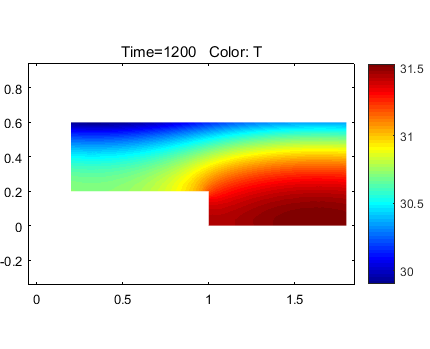
\includegraphics[width=7cm]{1200.png}
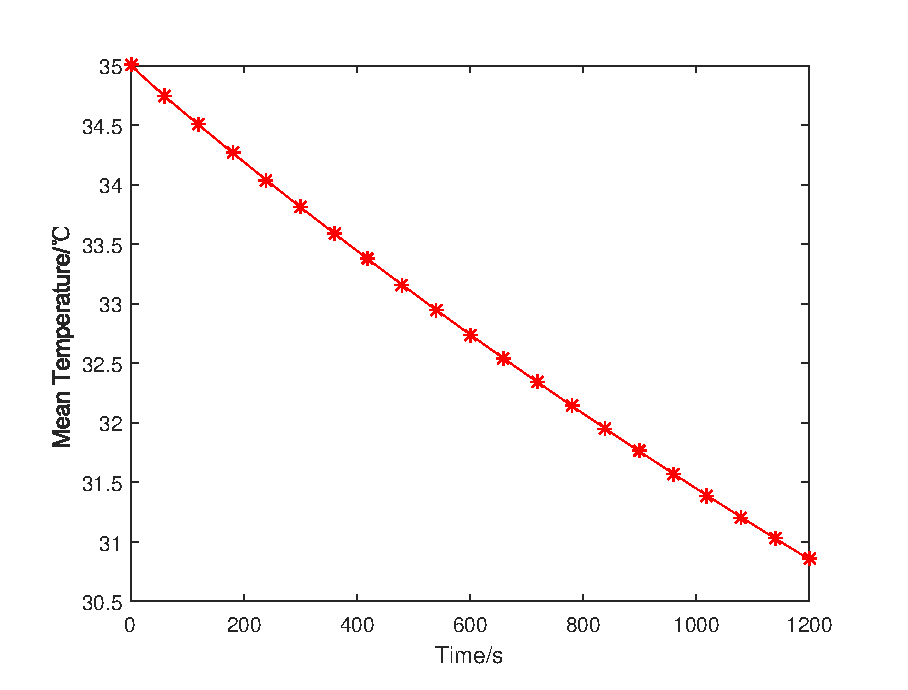
\includegraphics[width=7cm]{natrue.eps}
\caption{The free cooling process, with $M=600$}\label{nt}
\end{figure}

\section{Analysis of the Best Strategy}
Different people have different demands on taking bath in the bathtub. For example, some people
prefer to enjoy warm water early no matter how much hot water is used. Other people do not like the
difference of the temperature, maybe they also want to save water. Therefore, it is impossible to
point out which is more important: \emph{quantity}, \emph{stability}, or \emph{optimality}. In order
to put forward effective suggestions to consumers with different demands, we control two parameters,
temperature and flux from the faucet, to analyse the effect of different inflow plans. By analyzing
the graphs and linking them with normal lives, we can find some new methods to give consumers a
better experience.

In this section, we will set the initial temperature of water in the bathtub $T(0)=35^\circ$C to
simulate the situation by the problem sheet: the user begins to heat up the water when the water
\textbf{has been} cooled down.

\subsection{Different Temperature, Same Flux}
According to normal lives, we set the temperature in four levels, which are shown in \textbf{Table
\ref{show}}. It is usually impossible for the users to feel out the actual temperature of the water,
we also give a series of description to express the feeling of different levels of temperature. In
addition, we control the flux as $V_\mathrm{per}=$0.25L/s.
\begin{table}[!htbp]
\begin{center}
\caption{Levels of water temperature}
\begin{tabular}{cl}
    \toprule
    Temperature&Description\\
    \midrule
    38$^\circ$C&"Optimum temperature"\\
    40$^\circ$C&"A little higher temperature"\\
    42$^\circ$C&"Scalding temperature"\\
    45$^\circ$C&"Highest temperature"\\
    \bottomrule
\end{tabular}\label{show}
\end{center}
\end{table}

\paragraph{Optimum water}
By using PDE-Toolbox, we obtained the change in the bathtub by time for four kinds of water. We
calculated the mean temperature of the water in the bathtub in 20-minute-time, and the results are
shown in \textbf{Figure \ref{34}}. From the graph we can see and infer that by the increase of the
temperature, the water attaches the optimum temperature more and more early.
\begin{figure}[!htbp]
\small
\centering
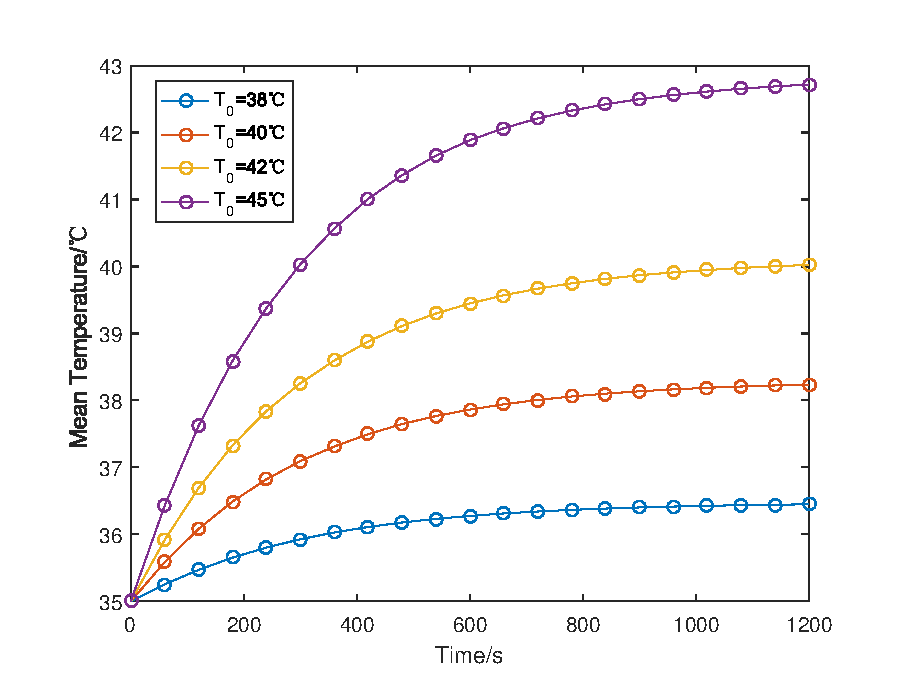
\includegraphics[width=10cm]{38404245.eps}
\caption{The mean temperature of bathtub water, with continuous inflow}\label{34}
\end{figure}

If we turn on the faucet from the beginning to the end, 38$^\circ$C and 40$^\circ$C water cannot
make the whole water attach the optimum temperature. So in the following concern about the
temperature, 38$^\circ$C and 40$^\circ$C inflow cannot heat up the water. However, if we choose
45$^\circ$C water, after a period of time, the water will be too hot to stand. For 42$^\circ$C
water, actually in the last 10 min, the temperature do not make any big influence.

Therefore, we thought out a new method. When the water attaches the optimum temperature, the user
cannot turn off the faucet. This can also help save the water. Based on the results before, we give
out three methods:
\begin{itemize}
    \item \textbf{Method 45 $\times$ 5}: Turn on the faucet with 45$^\circ$C inflow for 5min, and then
    turn off the faucet.
    \item \textbf{Method 42 $\times$ 5}: Turn on the faucet with 42$^\circ$C inflow for 5min, and then
    turn off the faucet.
    \item \textbf{Method 42 $\times$ 10}: Turn on the faucet with 42$^\circ$C inflow for 10min, and
    then turn off the faucet.
\end{itemize}

The mean value of the water with these methods is given in \textbf{Figure \ref{5m}}. From the graph
we can see that in the former 10 minutes, water in the bathtub keep the temperature in a comfortable
degree. However, along with the shut of the faucet, the temperature fell down at a quick speed. At
the time point of T=1200s, the temperature of Method $45\times5$ and Method $42\times5$ both fall
under 36$^\circ$C, which is not accepted. However, Method $42\times10$ gives a better performance in
maintaining the temperature in an acceptable level. So Method $42\times10$ is considered to be one
of the recommended strategies.
\begin{figure}[!htbp]
\small
\centering
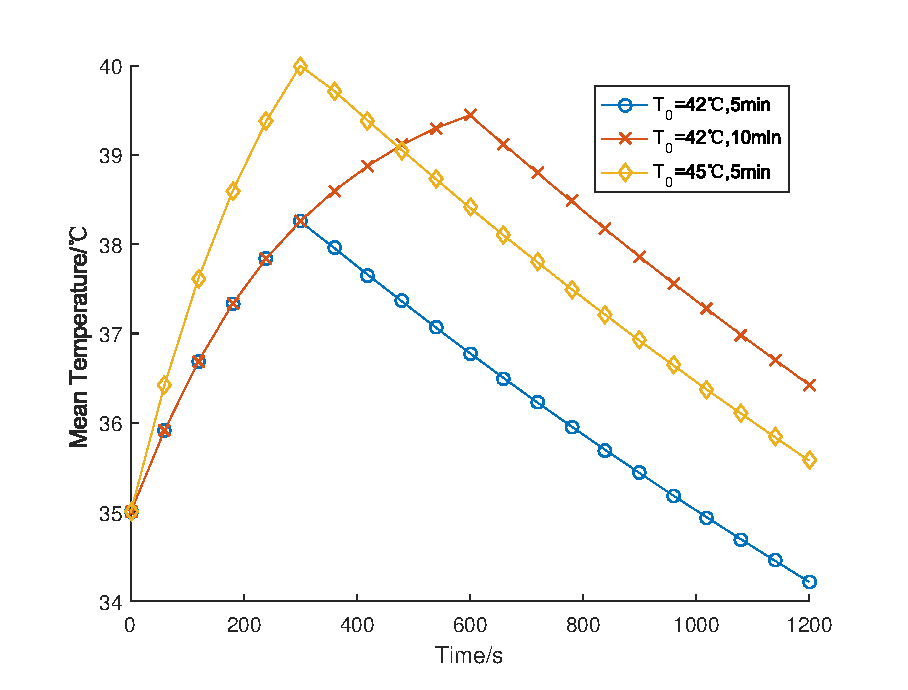
\includegraphics[width=10cm]{5min.eps}
\caption{The mean temperature of bathtub water, with a period of inflow}\label{5m}
\end{figure}

It is seen that the water will still cool down too early with only a period of inflow. So why not
turn on the faucet when the water fell down under the optimum temperature? Based on the results
before, we choose the two possible test two methods:
\begin{itemize}
    \item \textbf{Method 45-twice}: Turn on the faucet with 45$^\circ$C inflow for 5min, then turn
    off for 5min, and repeat such process once.
    \item \textbf{Method 42-twice}: The same as below, just with 42$^\circ$C inflow.
\end{itemize}

The mean temperature of water with these two methods is shown in \textbf{Figure \ref{ts}}. It shows
that Method 45-twice has a significant effect on the rising of the temperature. Compared with the
former method, Method 42-twice makes the water keep the temperature lower than the optimum
temperature for a period of time.
\begin{figure}[!htbp]
    \small
    \centering
    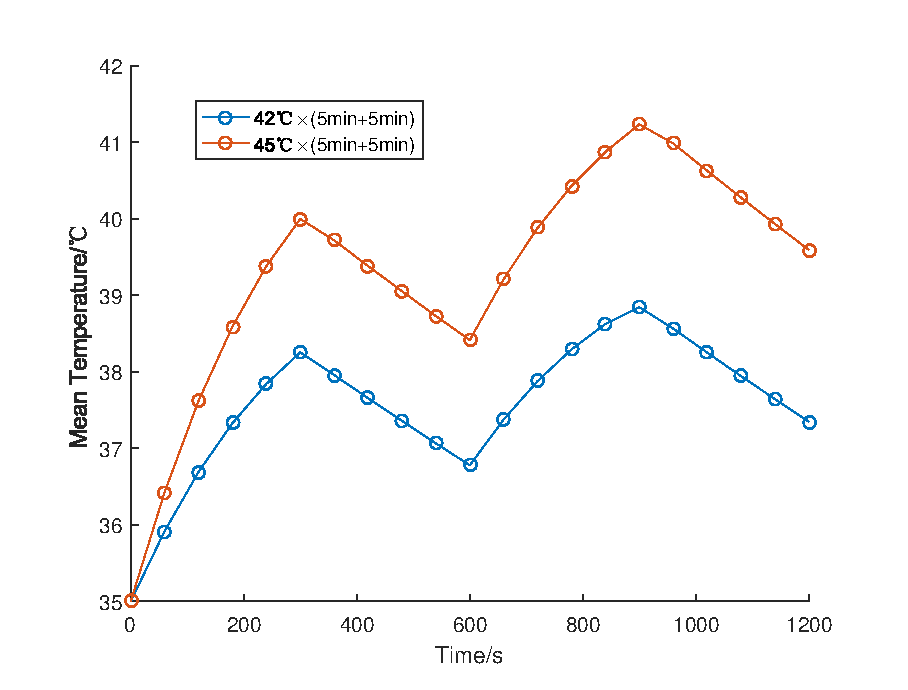
\includegraphics[width=10cm]{twice.eps}
    \caption{The mean temperature of bathtub water, with "twice"-methods}\label{ts}
\end{figure}


\paragraph{Uneven temperature}
We use standard deviation of the temperature data to evaluate the instability of the temperature.
Actually, the standard deviation of water may not represent the instability completely, for there is
always somewhere (near the faucet) with high temperature and somewhere (far from the faucet) with
low temperature. For example, if our feet and our arms are around 39$^\circ$C water and 37$^\circ$C
water all the time, respectively, maybe we would still not feel uncomfortable. Therefore the feeling
of uneven temperature while bathing may also be linked with the stability of the standard deviation
itself.

Firstly, we tested continuing inflow methods with various temperatures shown in \textbf{Table
\ref{show}}. The standard deviations of the temperature under these methods are shown in
\textbf{Figure \ref{s1}}. From the graph we can see and infer that by the increase of the
temperature, the standard deviation becomes larger and larger. That means hotter water will cause
more uneven temperature. In normal lives, temperature within 1.5 $^\circ$C difference is hard to be
felt. Therefore, 45$^\circ$C water may cause some trouble to people with high demand on uniform
temperature.
\begin{figure}[!htbp]
    \small
    \centering
    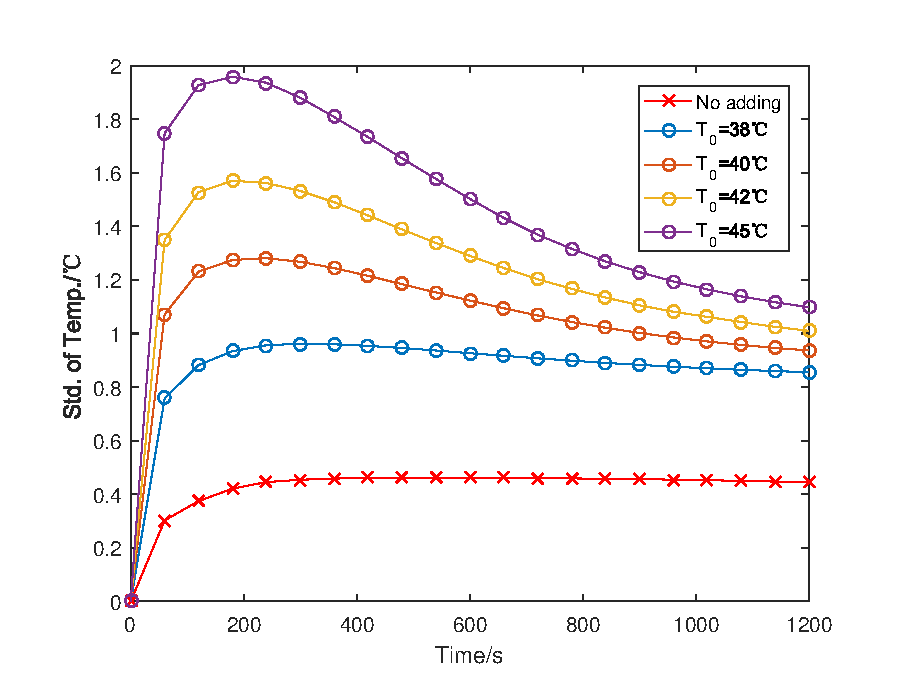
\includegraphics[width=10cm]{s38404245.eps}
    \caption{The standard deviation of the temperature, with continuous inflow}\label{s1}
\end{figure}

In addition, we also tested the "twice"-methods which we put forward before. The standard deviations
under the two methods, Method 45-twice and Method 42-twice, are shown in \textbf{Figure \ref{s2}}.
We can see that not only the standard deviation of water is a little lager, but the stability of the
standard deviation is much lower than the methods above. That is to say, discontinuous inflow may
cause "\emph{sometimes hot and sometimes cold}" water.
\begin{figure}[!htbp]
    \small
    \centering
    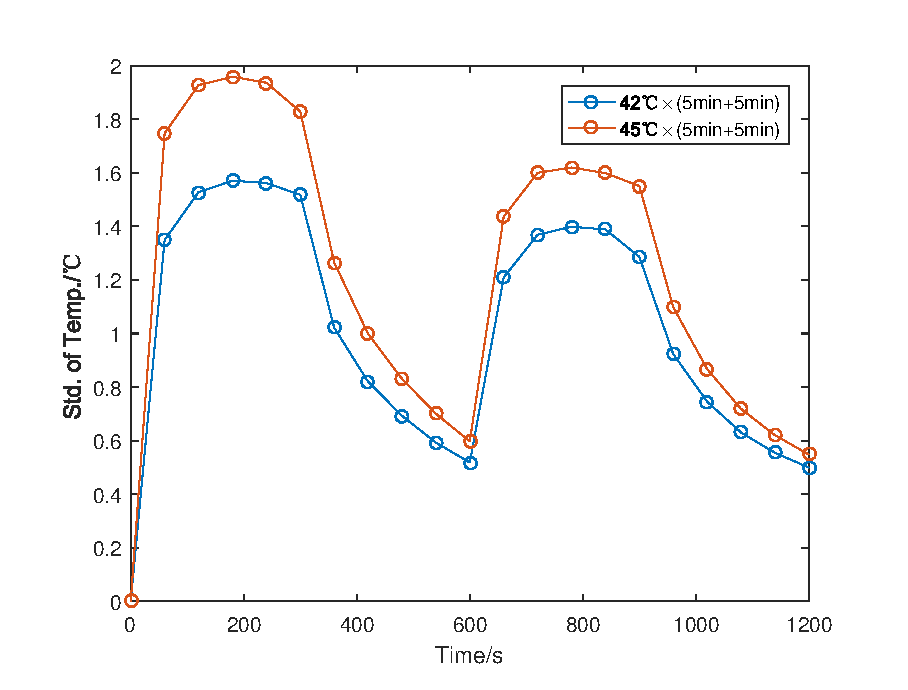
\includegraphics[width=10cm]{stwice.eps}
    \caption{The standard deviation of the temperature, under "twice"-methods}\label{s2}
\end{figure}

\subsection{Different Flux, Same Temperature}
Another parameter needs to control is the flux of inflow, which means turning on the faucet
"\emph{bigger}" or "\emph{thinner}". Here we give out the different flux which will be discussed
below in \textbf{Table \ref{vl}}. We also give a series of description about these choices, in order
to describe the actual motion on the faucet.
\begin{table}[!htbp]
\begin{center}
\caption{Levels of inflow flux}
\begin{tabular}{cl}
    \toprule
    Flux&Description\\
    \midrule
    No adding&"Faucet Off"\\
    0.025L/s (10\%)&"Trickle"\\
    0.15L/s (60\%)&"Turn on in half"\\
    0.25L/s (100\%)&"Maximum"\\
    \bottomrule
\end{tabular}\label{vl}
\end{center}
\end{table}
\paragraph{Optimum water}
By using PDE-Toolbox, we obtained the change in the bathtub by time for three kinds of flux of
inflow. The mean value of these methods are shown in \textbf{Figure \ref{ll}}. From the graph we can
see that by the increase of the flux, the water attaches the optimum temperature more and more
early. 10\%-flux method cannot keep the temperature increase, so it is eliminated. 60\%-flux and
100\%-flux method can attach the optimum temperature, but with 100\%-flux water all the time will
make water scalding.
\begin{figure}[ht]
\small
\centering
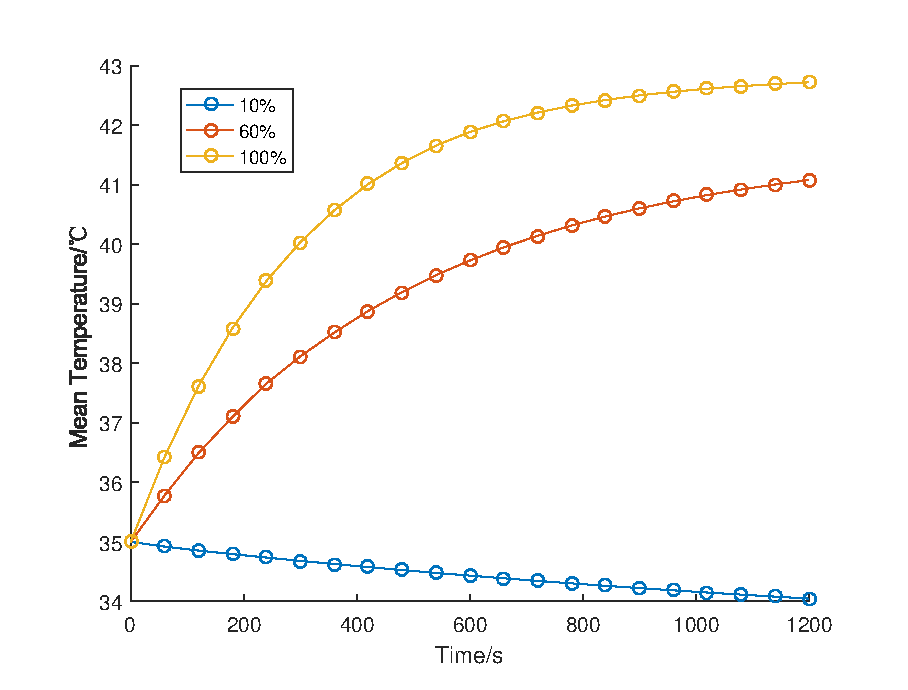
\includegraphics[width=10cm]{1060100.eps}
\caption{The mean temperature with continuous 45$^\circ$C inflow (different flux)}\label{ll}
\end{figure}

We also consider the effects of the temperature under the "twice"-methods. However, unlike the pair
before, we give such a pair of methods:
\begin{itemize}
    \item \textbf{Method 100\%-twice}: Turn on the faucet with 45$^\circ$C, 100\%-flux inflow for
    5min, then turn off for 5min, and repeat such process once.
    \item \textbf{Method 60\%-twice}: Turn on the faucet with 45$^\circ$C, 60\%-flux inflow for
    5min, then turn off for 5min, and repeat such process once.
\end{itemize}

The mean temperature of the water is shown in \textbf{Figure \ref{qt}}. The graph shows that inflow
with 100\% (maximum) flux can make the water keep the temperature around the optimum while 60\% flux
may make people feel a little cold at the beginning of the bath.
\begin{figure}[!htbp]
\small
\centering
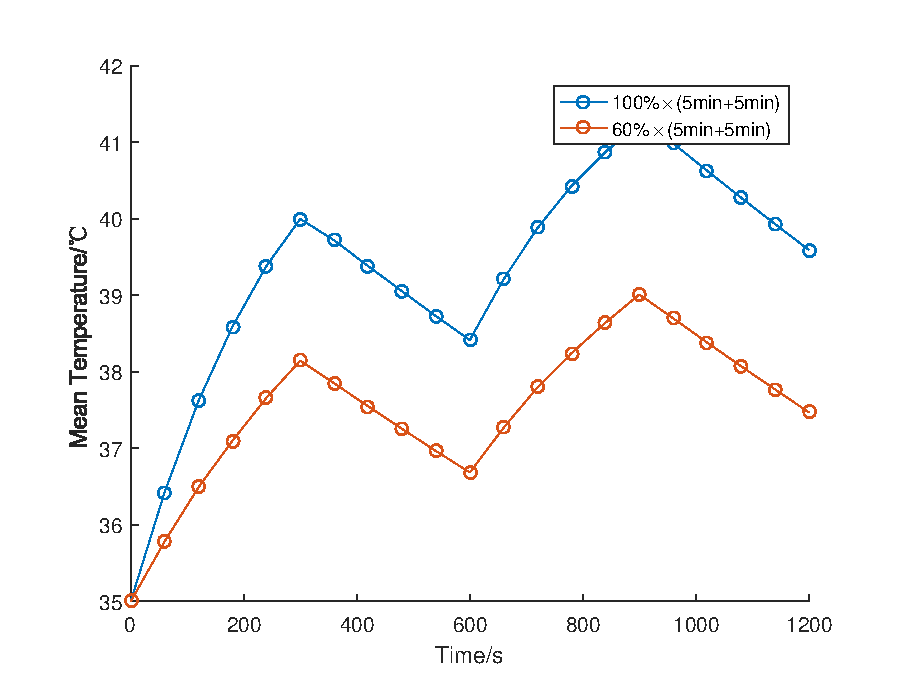
\includegraphics[width=10cm]{qt.eps}
\caption{The mean temperature with 45$^\circ$C inflow, under "twice"-methods}\label{qt}
\end{figure}

\paragraph{Uneven temperature}
We tested continuing inflow methods, and the results are shown in \textbf{Figure \ref{s3}}. From the
graph, we can see that by the increase of the flux, the standard deviation became more and more
larger, which is so say, more water per second from the faucet will cause more uneven temperature.
\begin{figure}[!htbp]
    \small
    \centering
    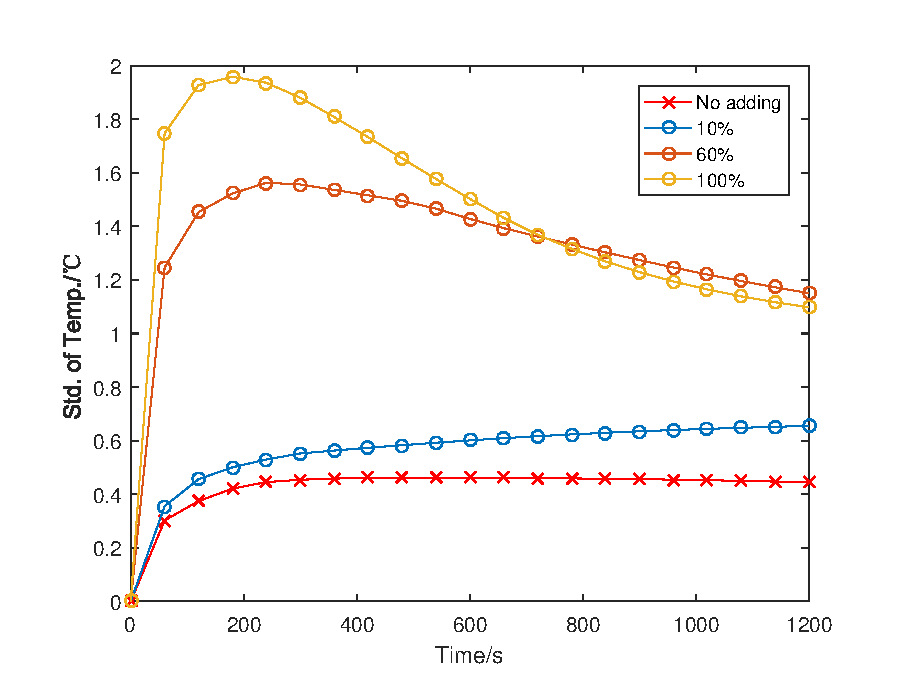
\includegraphics[width=10cm]{s_1060100.eps}
    \caption{The mean temperature with 45$^\circ$C inflow, under "twice"-methods}\label{s3}
\end{figure}

\subsection{Confirm the inflow methods}
From the analysis above, we have gained two feasible methods: Continuous water inflow with lower
temperature, and Method 42$\times$10. There are also two kinds of "twice"-methods which are
feasible, but here we will give two more kinds of methods. Actually, both the increase of inflow
temperature and flux have the same effect on the whole water (based on our research). In normal
lives, we usually open the faucet for water with high temperature and big flux to heat the water at
the beginning. When the temperature falls down after we relax for a period of time, we often turn on
the faucet and let water with warm temperature and mediate flux enter the bathtub to keep the
temperature. Therefore, we also make two more effective methods to add in the final list. So we have
four feasible methods, which are:
\begin{itemize}
    \item \textbf{Method 42}: Continuous 42$^\circ$C water inflow;
    \item \textbf{Method 42$\times$10}: Turn on the faucet with 42$^\circ$C inflow for 10min,and
    then turn off the faucet.
    \item \textbf{Method 45+42}: Turn on the faucet with 45$^\circ$C inflow for 5min, and then turn
    off. Turn on with 42$^\circ$C inflow 5min later, still for 5min.
    \item \textbf{Method 45+42-little}: As same as the method before, but the 42$^\circ$C inflow is
    with 60\% flux.
\end{itemize}

We tested the four methods about the "optimum temperature" and "uneven temperature", and the results
are shown in \textbf{Figure \ref{strategy}} (mean and std. of temperature). From the graph we can
see that \textbf{Method 42} can lead to more optimum and uniform temperature, but this method waste
a lot of water. \textbf{Method 45+42} will save a lot of water , meanwhile the temperature is more
uneven. \textbf{Method 42$\times$10} cannot give very comfortable water in the end of the bath.
Compared with the three methods above, \textbf{Method 45+42little} is a mediate strategy.
\begin{figure}[!htbp]
\small
\centering
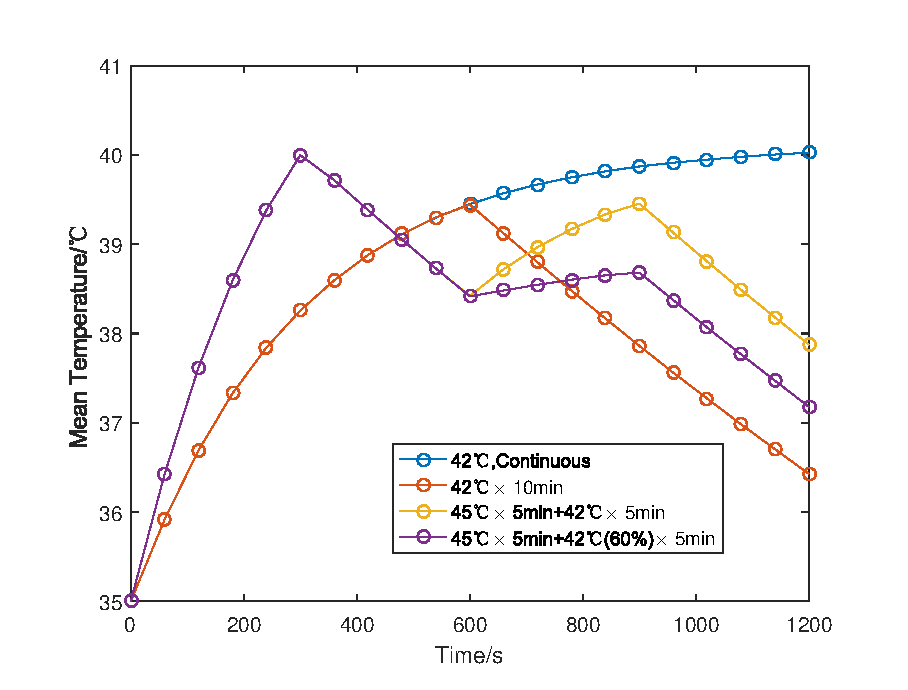
\includegraphics[width=7.3cm]{strategy.eps}
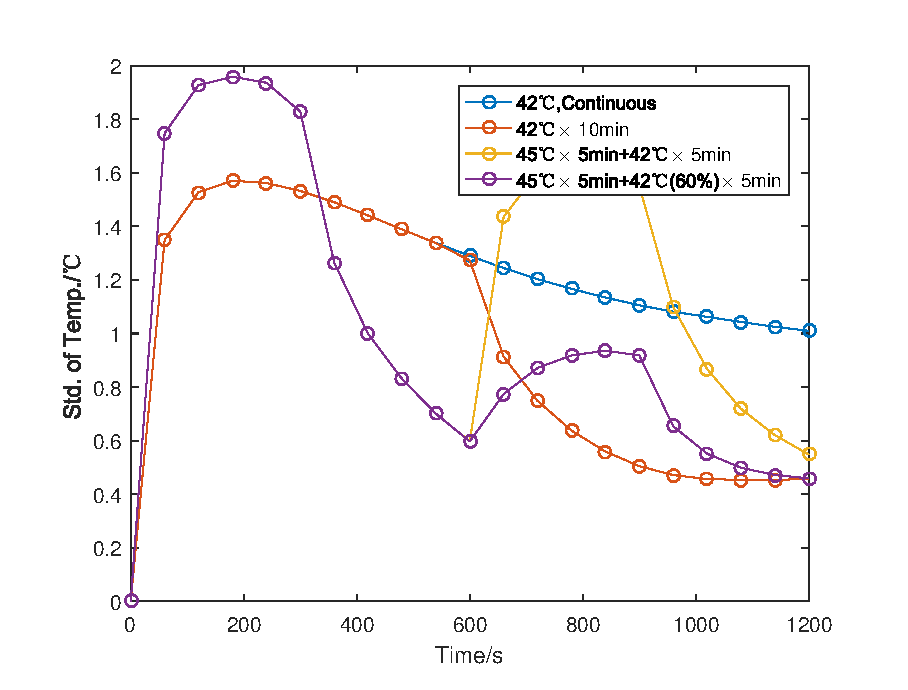
\includegraphics[width=7.3cm]{s_strategy.eps}
\caption{The mean and std. of temperature, under the four recommended methods}\label{strategy}
\end{figure}

Actually, the users can make their choices neatly according to their demands. According to the
results, we give our suggestion in \textbf{Figure \ref{check}}.
\begin{figure}[!htbp]
\small
\centering
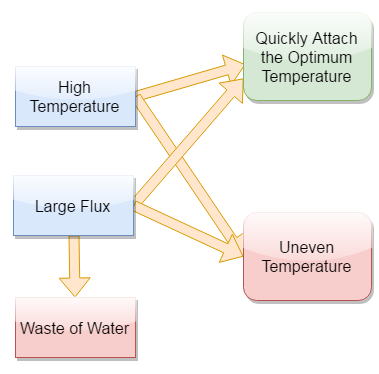
\includegraphics[width=7cm]{check.png}
\caption{Diagram of actions \& results}\label{check}
\end{figure}


\section{Analysis of Various Conditions}\label{condition}
We simplify our time-space based temperature model by setting down the shape volume and material of
the bathtub,the position of the faucet,the shape, volume and temperature of the person and assuming
that the person is static. But there are multiple kinds of bathing in real life, and different kinds
of people may have different strategies to have a better experience. So in this part, we use our
model to determine the extent to which our strategy depends on the complex and multiple factors in
order to give corresponding and optimum suggestions on different conditions.

Another way to say, we change several parameters' value in the model to make a \textbf{sensibility
analysis}.

\subsection{The Factors of the Bathtub}
There are four factors of the bathtub which can affect the effects of different strategies and
determine the best strategy: shape,volume,material and the position of the faucet.

\paragraph{Shape}For the shape of the bathtub, we divide the bathtubs into two kinds based on the
shape of their bottom: plane-style (which has been studied before) and concave-style. Under the
prerequisite of having the same volume, we reshape the regular plane-style bathtub to build a
concave-style bathtub. The image of the cross section is shown in shown in \textbf{Figure
\ref{bathtub}}. Based on the parameters before, we test the free cooling process of concave-style
bathtub, which can illustrate the actual influence made by the difference of shape. The results
(mean temperature and std. of temperature) are shown in \textbf{Figure \ref{s4}}, which shows that
two curves are almost coincided. That means the extent of the model depends little on the shape of
the bathtub.
\begin{figure}[!htbp]
\small
\centering
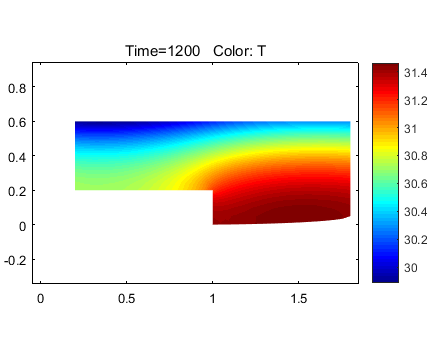
\includegraphics[width=7cm]{m2.png}
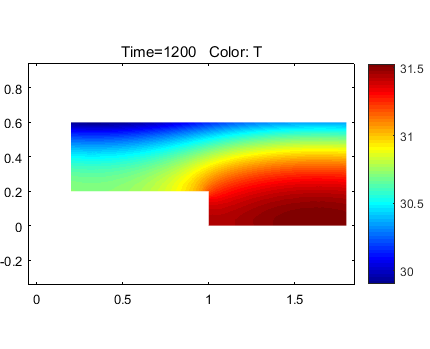
\includegraphics[width=7cm]{1200.png}
\caption{The concave-style bathtub together with the plane-style one}\label{bathtub}
\end{figure}

\begin{figure}[!htbp]
\small
\centering
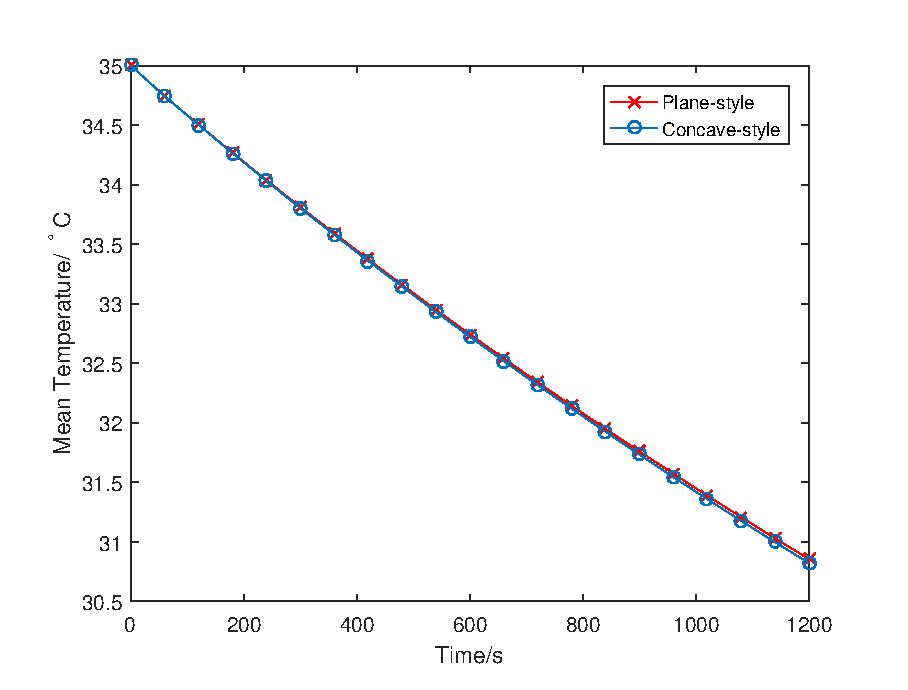
\includegraphics[width=7cm]{TY.eps}
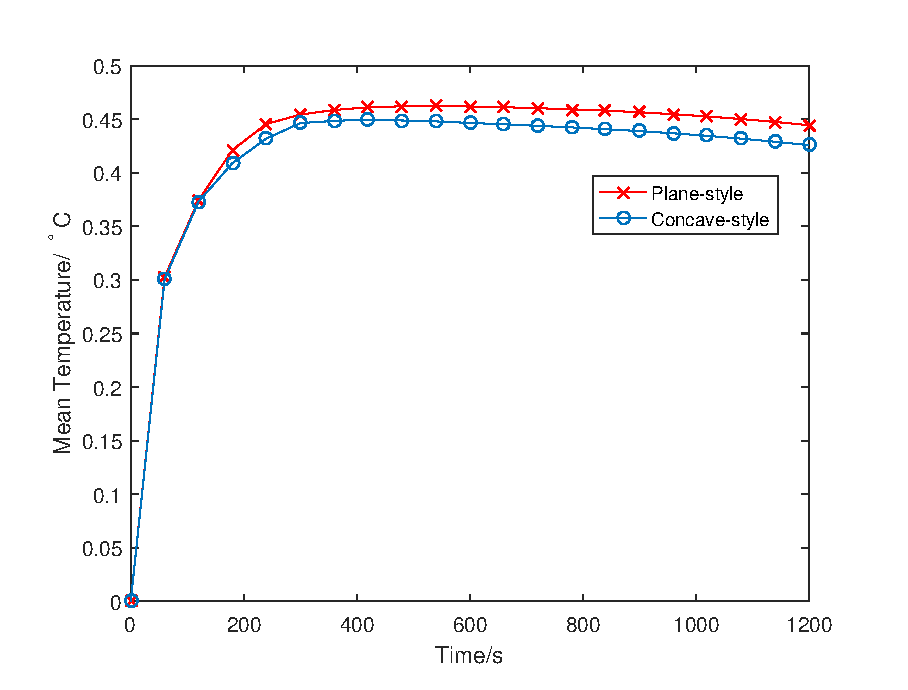
\includegraphics[width=7cm]{sTY.eps}
\caption{The mean and std. of the temperature in concave-style and plane-style bathtub}\label{s4}
\end{figure}


\paragraph{Volume}To judge how much the effect of strategy is influenced by the volume of the
bathtub, we choose two particular size of the bathtub. The \textbf{regular} size is as same as
before (1.8m$\times$0.8m$\times$0.6m), while the \textbf{smaller} size is defined as
1.5m$\times$0.6m$\times$0.5m. As two typical instances, we test these two kinds of volume under two
methods: nature cooling process, and continuous 42$^\circ$C inflow (Method "42", which is a feasible
method in the normal bathtub).

The mean temperature in different situations are shown in \textbf{Figure \ref{s5}}. We can see that
the temperature rise up falls down more quickly under the same method when using a smaller bathtub.
We can see that the method is still effective to the small bathtub, which proves that our model
depends not much on the flux of the bathtub. However, the \emph{details} of the recommended methods
such as temperature or inflow flux, are supposed to have some slight changes in a smaller bathtub.
\begin{figure}[!htbp]
\small
\centering
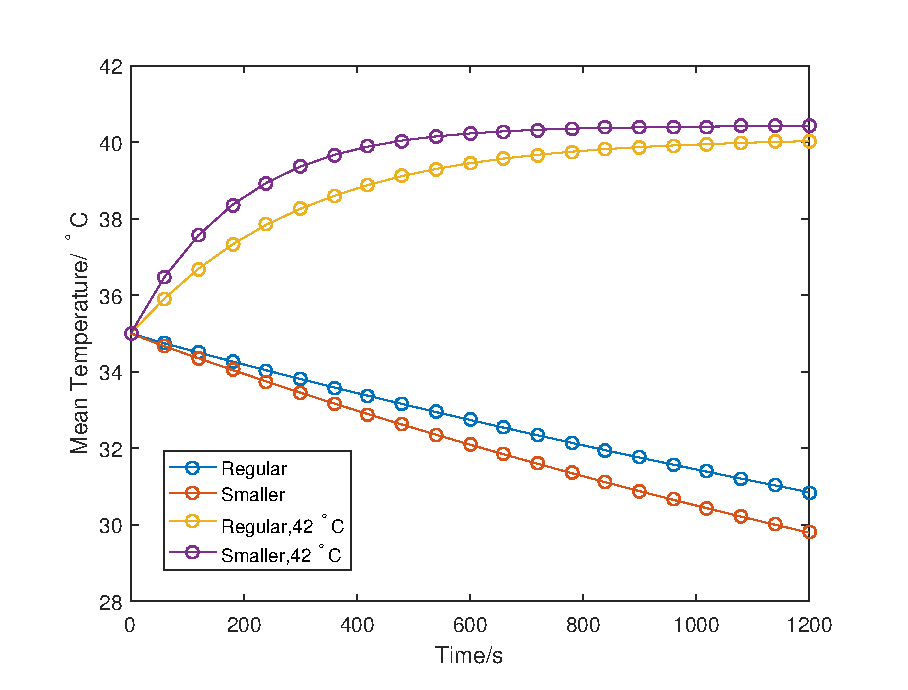
\includegraphics[width=10cm]{Smaller.eps}
\caption{The mean temperature in regular and smaller bathtub}\label{s5}
\end{figure}

\paragraph{Material}Different material can cause differences in the coefficient $k$ of thermal
conduction, which is defined in Section \ref{k}. However, the thermal conductivity coefficient
values of different materials are small, considering the fast loss through the water surface. So
materials make little difference on the thermal conduction and we can infer that the strategy has
small dependence on material based on the analysis above.

\paragraph{The Position of the Faucet}We consider two kinds of the faucet's position: one is in the
\emph{upper corner}, while the other is in the \emph{upper center} which is used in the bathtub
studied before. We assume that the faucet would not in the same side of the person.(Who will let the
burning water pouring on his or her back?) And we simulate the two conditions under \textbf{Method
42} in PDE-Toolbox.

The distribution of temperature with two different positions are shown in \textbf{Figure
\ref{center}}, and the mean and std. of temperature under different conditions are shown in
\textbf{Figure \ref{mc}}. The two graphs show that if the faucet is in the upper corner, the water
is at a lower temperature (under 38 $^\circ$C), and it can cause more uneven temperature. If the
faucet settles at the central side (upper center) of the bathtub, it is better for comfortable bath
experience, since the whole bathtub is symmetrical and the heat is concentrated in the center of the
bathtub.
\begin{figure}[!htbp]
\small
\centering
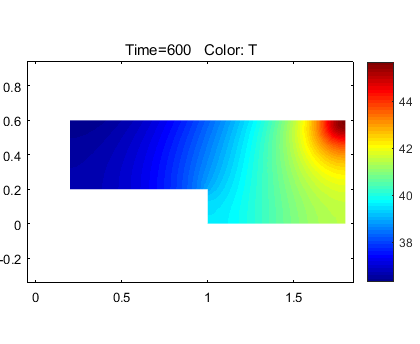
\includegraphics[width=7cm]{side.png}
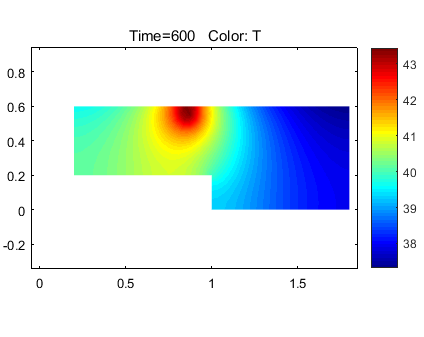
\includegraphics[width=7cm]{center.png}
\caption{The temperature distribution with different position of faucet ($T=600$s)}\label{center}
\end{figure}

\begin{figure}[!htbp]
\small
\centering
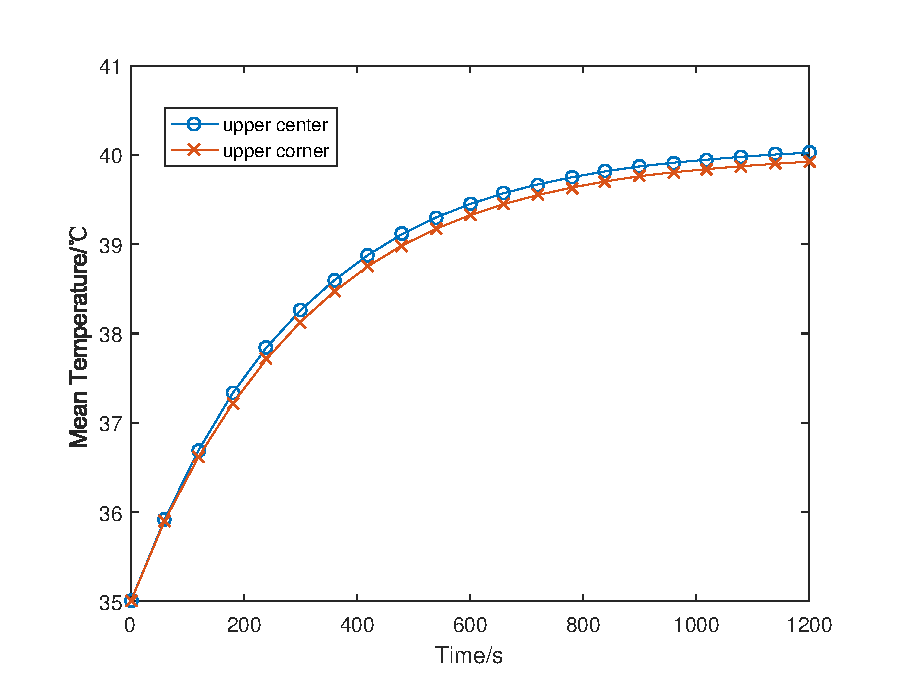
\includegraphics[width=7cm]{cc.eps}
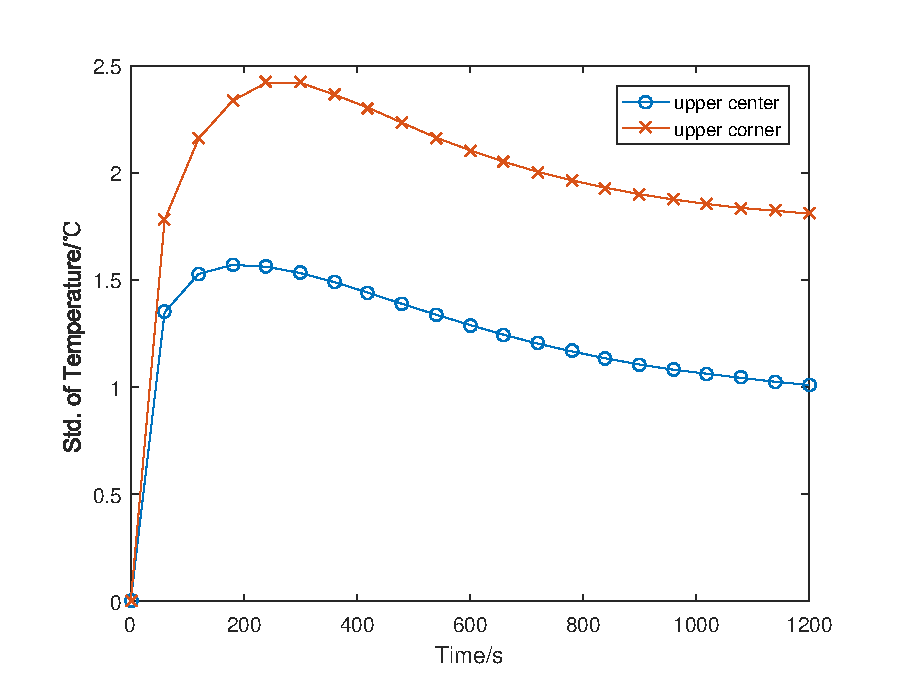
\includegraphics[width=7cm]{s_cc.eps}
\caption{The mean and std. of temperature with different position of faucet}\label{mc}
\end{figure}

Generally speaking, the position of faucet makes a big difference on the strategy, and the upper
center position of the faucet is more likely to provide a better bath experience with optimum and
uniform temperature. So in fact, most of the bathtubs have their faucets on the central side, which
is shown in \textbf{Figure \ref{fact}}.
\begin{figure}[!htbp]
\small
\centering
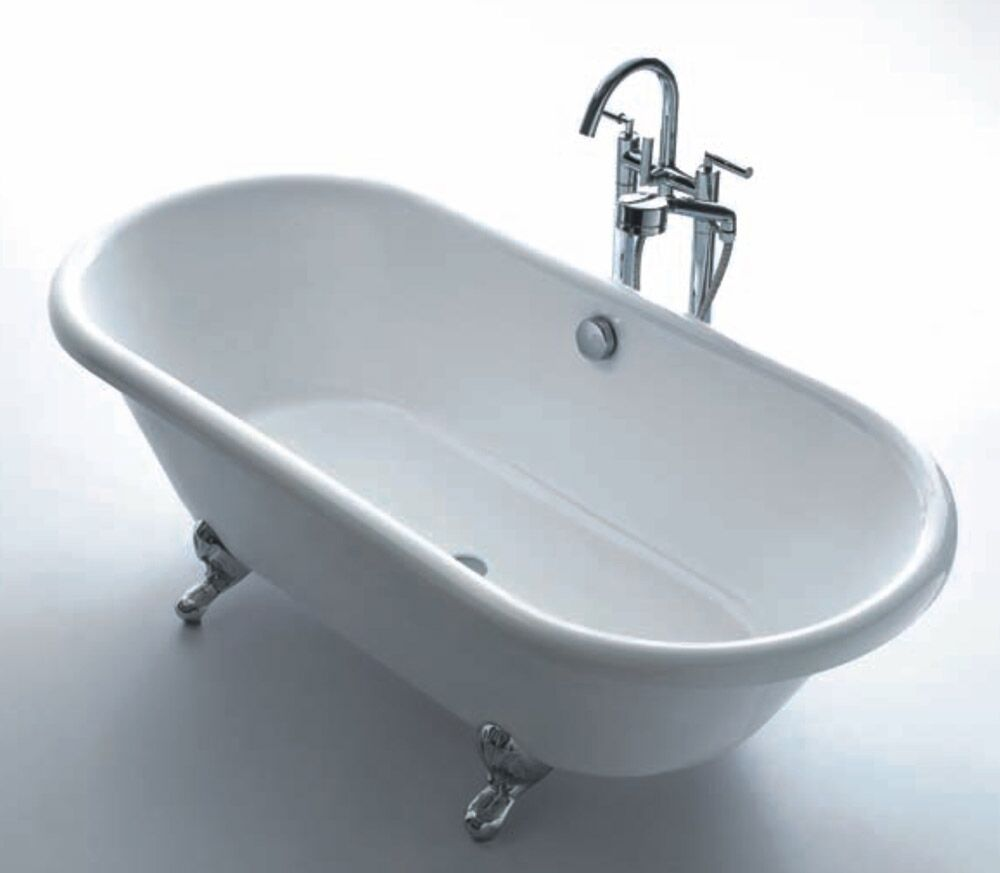
\includegraphics[width=8cm]{123.jpg}
\caption{A typical bathtub with faucet on central side}\label{fact}
\texttt{http://useful999.com/product/image/pics/LS-170B.jpg}
\end{figure}



\subsection{The Factors of the person}
Different people may have different suitable strategy to take a comfortable bath, the main factors
are shape which means the posture of the person, volume, temperature of the human body and motions.
And we would analyse the extent which our strategy depends on them one by one.

\paragraph{Shape}The effect caused by human body is not so much in the temperature changing process,
so we think that the different of the human shape will not make a difference in the recommended
strategies.

\paragraph{Volume}Since the volume of the person affect the volume of water and further reflect the
volume of the bathtub, we think that the effects of the volume of the person is similar to those of
the volume of the bathtub. So following the previous results about the volume of the bathtub, we can
infer that the strategy has small dependence on the volume of the person based on the analysis of
the volume of the bathtub.

\paragraph{Temperature}The temperature of the person would not have a great impact on the strategy
for the following reasons:
\begin{enumerate}[\bf 1.]
    \item The heat transfer coefficient between the human body and water is too tiny so that the
    heat transfer effects are inconspicuous;
    \item The person is almost exothermic and at a constant temperature.
\end{enumerate}
We can infer that the strategy may rely less on the temperature of the person.

\paragraph{Motions}Since the motions of the person are too complex and various to analyse, we can
quantify the effects of the motions through the changes of parameter. Based on the heat transfer and
heat convection theories, the motions of the person would increase the heat transfer coefficient and
the heat convection coefficient. It means that the motions accelerate heat transfer,and the
temperature would decline rapidly and acutely. We can infer that the best strategy rely on the
motions slightly, and more specifically, higher temperature of inflow will be necessary.

\subsection{A Bubble Bath Additive}
A bubble bath additive is a kind of surfactant which is compound that lower the surface tension (or
interfacial tension) between two liquids, between a gas and a liquid.Surfactants can form a foam,
facilitate the removal of dirt, and enable the mixture of water and oil. From the view about the
reduction of the surface tension, adding some bubbles can increase the evaporation of water.

However, shampoo bubbles have very large surface areas with very little mass. The bubbles prevent
the heat transmission a lot between the water and the outside environment. And compared to the
increasing evaporation, the reduction of heat transmission occupies the dominant place. Therefore, a
bubble bath can keep the temperature more stable than a normal bath. The bathing strategies change
towards less flux, less time and lower temperature in a corresponding way.

\textbf{Figure \ref{bubble}} shows the photograph of a bathtub with bubbles and the diagram of how
bubbles slow down the cooling process.
\begin{figure}[!htbp]
    \small
    \centering
    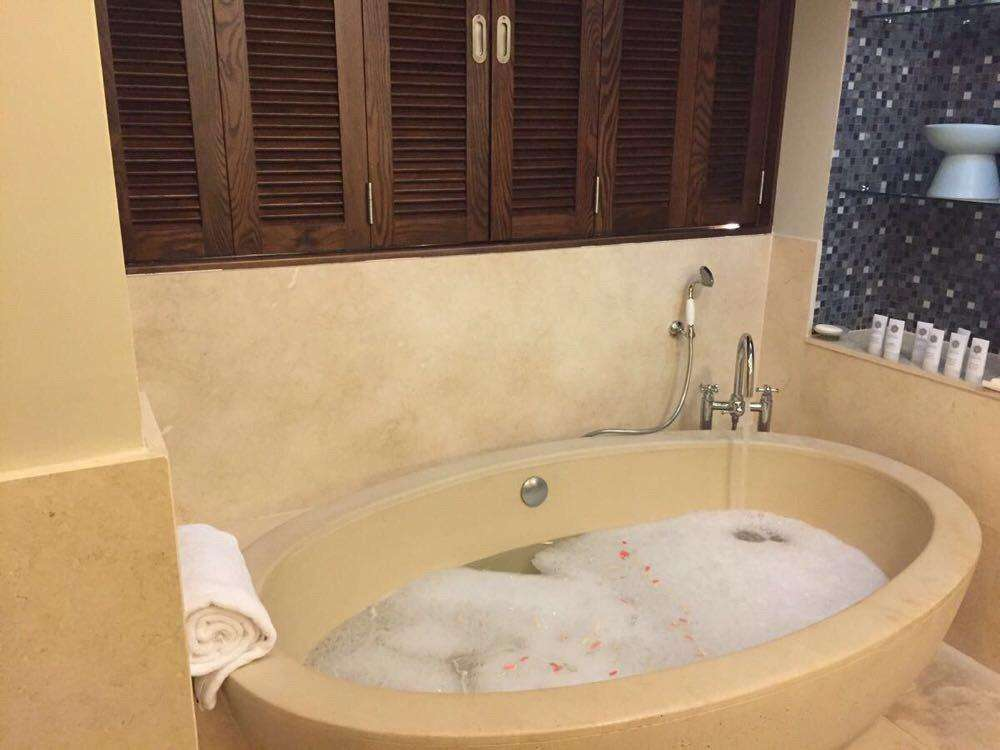
\includegraphics[width=7cm]{picture.jpg}
    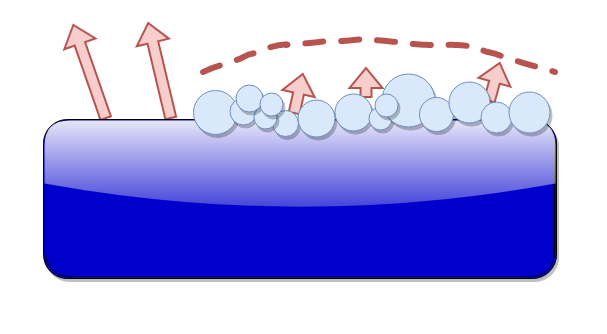
\includegraphics[width=7cm]{paopao.png}
    \caption{A bathtub with bubbles and the diagram about the effect of bubbles}\label{bubble}
    source of the photograph: \texttt{http://you.ctrip.com/travels/mauritius444/2355353.html}
\end{figure}

\subsection{New Consideration: Different Initial Temperature}
In the original problem, the user heat up the water after the water in the bathtub has cooled down,
so we set the initial temperature as 35$^\circ$C. If we do not follow the original problem and
suppose that the user turn on the faucet when the water is still at the optimum temperature, is
there anything to be different?

To find out the answer, we assume that the initial temperature is 38 $^\circ$C (The optimum
temperature). We test two methods with continuous inflow:
\begin{enumerate}[\qquad \bf 1.]
    \item \textbf{Method 40}: Continuous 40 $^\circ$C inflow, with 100\%-flux (0.25L/s).
    \item \textbf{Method 42-little}: Continuous 42$^\circ$C inflow, with 60\%-flux (0.15L/s).
\end{enumerate}
We test these two methods under such condition, and compare the results with the data under the
former condition ($T_0=35^\circ$C), Method 40. The mean temperature in these three situations are
shown in \textbf{Figure \ref{38}}. We can see that Method 40 and Method 42-little can both keep the
temperature, while these two methods are unrecommended when the initial temperature is 35$^\circ$C.
And from the change of the curves we can see that adding water earlier can keep the temperature more
uniform. So we can see that when consumers enter the bathtub, maybe turning on the faucet directly
is a better choice, comparing with turning it on when the water is not hot enough any longer.
\begin{figure}[!htbp]
\small
\centering
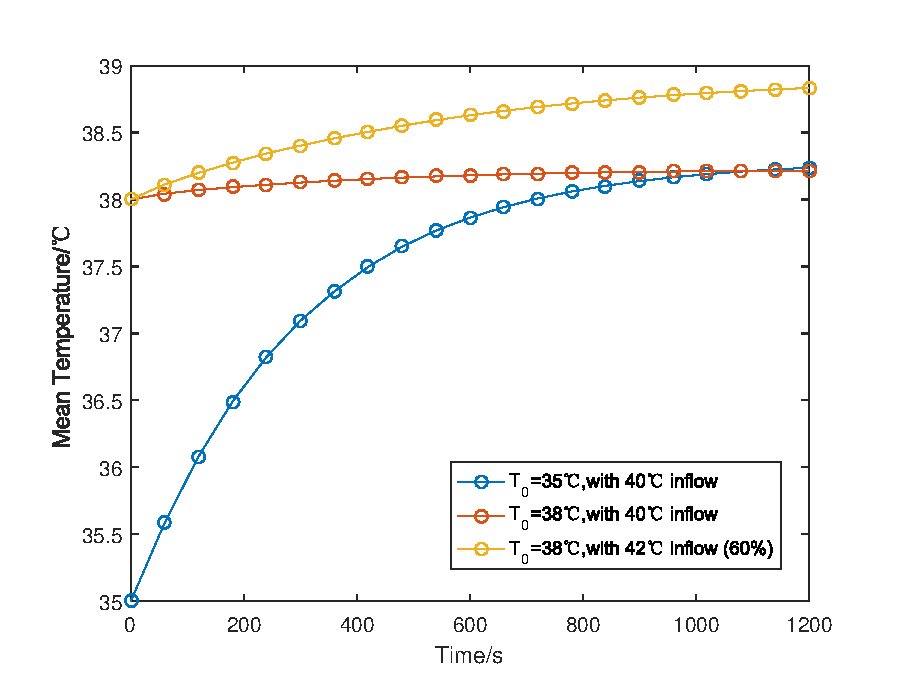
\includegraphics[width=10cm]{T38.eps}
\caption{The mean temperature of the water, with different initial temperature and methods}
\label{38}
\end{figure}

\section{Conclusion}
In this study, we construct the Time-Space Based Temperature Model through PDE-Method to give
consumers effective strategies of having a bath in the bathtub. We control two parameters,
temperature and flux of inflow, to find out how these parameters influence the effect of the inflow.
In the end, we give four recommended methods to get optimum and uniform temperature while not
wasting too much water, which are \textbf{Method 42}, \textbf{Method 42$\times$10}, \textbf{Method
45+42} and \textbf{Method 45+42-little}.

By examining the model with the change of some parameters, our model depends little on the
shape/volume/material of the bathtub and the shape/volume/temperature of the person. If the position
of the faucet is changed, it is proved that attaching the same demand on temperature by this bathtub
will waste more water than our initial bathtub. In addition, a bubble bath will keep the temperature
of the water in a certain extent because of the prevention of water's evaporation.

Different methods may show different ranks of effect according to the users' demand, the conditions
outside the bathtub and of the bathtub, and so on. However, according to our research in Section
\ref{condition}, these recommended methods are still useful under various conditions, if the details
(e.g. the temperature and the time of period) are properly adjusted. So the users can choose and
adjust the bath strategy based on the rules below:

\paragraph{Rule I}
\emph{High temperature and large flux can make the water attach the optimum temperature earlier,
meanwhile it may cause uneven temperature and waste of water.}
\paragraph{Rule II}
\emph{Evenness comes from continuous inflow with appropriate temperature, a little higher than the
optimum temperature in usual.}
\paragraph{Rule III}
\emph{The best strategy to have an excellent bath is to heat up the water before it cool down.}

\section{Strengths and Weaknesses}
\subsection{Strengths}
\begin{itemize}
    \item The model can reflect the change of temperature in every place of the bathtub, when the
    parameters of bathtub,people and water are input in the model.
    \item Through the analysis of the static temperature pattern with a continuous heat producer,
    our model successfully simulate the temperature's change with the water flow, with the help of
    our adjusting some parameters in order to correspond the real condition.
    \item Our model do not give only one strategy while bathing which may restrict the consumers'
    "freedom". According to different consumers's demand about the water, our model can give
    specific and effective strategies.
\end{itemize}

\subsection{Weaknesses}
\begin{itemize}
    \item The model use the cross section of the bathtub to analyze the temperature of the water.
    However,the shape of the bathtub can't make sure that each section is the same,and with the
    consideration of different people's shape, there must be some deprivation of our results.
    \item Some parameters in our model (such as the thermal conductivity between two materials) are
    adjusted several times by using PDE-toolbox in the MATLAB for there is no research that give
    these parameters certain values. The value of these parameters in our model may have some
    deprivation from the real value.
\end{itemize}

\clearpage
{\renewcommand{\baselinestretch}{1.3}\normalsize
\section*{Report for the Users}\addcontentsline{toc}{section}{Report for the Users}
\begin{flushleft}
Dear users:
\end{flushleft}

Thank you very much for choosing our bathtubs. Each piece of your support is our valuable treasure
which can encourage us to develop better bathtubs.We express our sincere thanks to you and your
family!
For this kind of bathtub, we have some suggestions for you:
\begin{enumerate}[\bf 1.]
    \item You don't have to worry about the full-water condition, because when the bathtub is full
    of water, the overflow drain can drain out the excess water.
    \item With the consideration that you will have your special demands on the bath water, we give
    you some suggestion through \textbf{Table \ref{advices}} so that you can choose what you prefer
    (or just freestyle you bath).
    \begin{table}[!htbp]
    \centering
    \footnotesize
    \caption{Various strategies (assumption: bath time is 20 minutes)}
    \label{advices}
        \begin{tabular}{c|ccc|c|c}
        \toprule
        \multirow{2}{*}{} & \multicolumn{3}{c|}{Method}
         & \multirow{2}{*}{Comfortability} & \multirow{2}{*}{Water use}\\
        \cline{2-4} & \multicolumn{1}{c|}{Temperature} & \multicolumn{1}{c|}{Volume}
        & Time & {} & {}\\
        \midrule
        \multirow{3}{*}{Turn on the faucet when} & \multicolumn{1}{c|}{scalding}
         & \multicolumn{1}{c|}{maximum} & continuous & high & large\\
        \cline{2-6} & \multicolumn{1}{c|}{scalding} & \multicolumn{1}{c|}{maximum}
         & on for 10min & middle & middle\\
        \cline{2-6} & \multicolumn{3}{c|}{highest-maximum-on for 5min,}
         & \multirow{2}{*}{middle} & \multirow{2}{*}{middle}\\
        \multirow{3}{*}{you enter the bathtub}
         & \multicolumn{3}{c|}{scalding-maximum-on for 5min later}{} & {} & \\
        \cline{2-6} & \multicolumn{3}{c|}{highest-maximum-on for 5min,}
         & \multirow{2}{*}{middle} & \multirow{2}{*}{small}\\
        {} & \multicolumn{3}{c|}{scalding-half-on for 5min later} & {} & {}\\ 
        \midrule
        Turn on the faucet when & \multicolumn{1}{c|}{a little higher}
         & \multicolumn{1}{c|}{maximum} & continuous & high & large\\
        \cline{2-6} you feel the water is cold & \multicolumn{1}{c|}{scalding}
         & \multicolumn{1}{c|}{half} & continuous & high & middle\\
        \bottomrule
        \end{tabular}
    \end{table}
    \item You can turn off the faucet 5min before you get out the bathtub, which can save a lot of
    water. Our bathtubs' ability of heat preservation is not too weak!
\end{enumerate}

However, for there is a significant difference of temperature between the bathtub inside and
outside, we can't promise that the water has an evenly maintained temperature throughout the
bathtub.It is very difficult to keep the near-faucet place's temperature the same as the
far-from-faucet place's.We are very sorry for the trouble caused by our bathtubs.
}





\showReference
\end{document}
